
\documentclass[aspectratio=169]{beamer}

\usepackage[utf8]{inputenc}
\usepackage[T1]{fontenc}
\usepackage[ngerman]{babel}
\usepackage{media9}
\usepackage{graphicx}
\usepackage{booktabs}
\usepackage{listings}
\usepackage{xcolor}
\usepackage{textgreek}
\usepackage[absolute, overlay]{textpos}
\usepackage{hyperref}
\setlength{\TPHorizModule}{\paperwidth}
\setlength{\TPVertModule}{\paperheight}
\TPGrid{1}{1}
\usetheme{Madrid}
\setbeamertemplate{frametitle}{}
\usecolortheme{default}

\definecolor{codegreen}{rgb}{0,0.6,0}
\definecolor{codegray}{rgb}{0.5,0.5,0.5}
\definecolor{codepurple}{rgb}{0.58,0,0.82}
\lstdefinestyle{mystyle}{%
    commentstyle=\color{codegreen},
    keywordstyle=\color{magenta},
    numberstyle=\tiny\color{codegray},
    stringstyle=\color{codepurple},
    basicstyle=\ttfamily\footnotesize,
    breakatwhitespace=false,
    breaklines=true,
    captionpos=b,
    keepspaces=true,
    numbers=left,
    numbersep=5pt,
    showspaces=false,
    showstringspaces=false,
    showtabs=false,
    tabsize=2
}
\lstset{style=mystyle}



% --- METADATA ---
\title{02 Algorithmik Asymptotische Analyse}
\author[Daniel Gaida]{Daniel Gaida}
\institute{Prof. Dr. Daniel Gaida \\ Professor für Cyber-Physische Systeme \\ Fakultät für Informatik und Ingenieurwissenschaften - Institut für Informatik}
\date{17.07.2021}

\begin{document}

\setbeamertemplate{footline}{} 
\setbeamertemplate{navigation symbols}{}
\begin{frame}
  \titlepage
\end{frame}


% --- Slide 1 ---
\begin{frame}[fragile]
\begin{textblock}{0.885}(0.099, 0.022)
  \begin{minipage}[b][0.031\paperheight]{\linewidth}
    \raggedright
    \fontsize{3}{3.3}\selectfont Algorithmik – Laufzeitanalyse von Algorithmen durch Asymptotische Notation
  \end{minipage}
\end{textblock}
\begin{textblock}{0.886}(0.099, 0.076)
  \begin{minipage}[t][0.131\paperheight]{\linewidth}
    \textbf{Lernraum I: Abstrakte Datentypen, Datenstrukturen und Asymptotische Notation}
  \end{minipage}
\end{textblock}
\begin{textblock}{0.886}(0.099, 0.226)
  \begin{minipage}[t][0.63\paperheight]{\linewidth}
    {\scriptsize
    \begin{itemize}
      \item Abstrakte Datentypen
      \item Liste, Stapel, Warteschlange, Tabelle (Dictionary)
      \item Datenstrukturen
      \item Array, Verkettete Liste
      \item Implementierungen der Abstrakten Datentypen mit den Datenstrukturen …
      \item Array
      \item Verkettete Listen
      \item Analyse von Laufzeit und Speicherbedarf der Implementierungen
      \item O-Notation
      \item Laufzeitanalyse von Algorithmen durch Asymptotische Notation
      \item O-Notation, Ω-Notation, Θ-Notation
      \item Fallanalyse: Worst Case, Best Case Analyse
      \item Laufzeitanalyse von Rekursiven Algorithmen durch Asymptotische Notation
    \end{itemize}
    }
  \end{minipage}
\end{textblock}
\begin{textblock}{0.106}(0.099, 0.877)
  \begin{minipage}[b][0.026\paperheight]{\linewidth}
    \raggedright
    \fontsize{3}{3.3}\selectfont 06.03.2026
  \end{minipage}
\end{textblock}
\begin{textblock}{0.106}(0.099, 0.928)
  \begin{minipage}[b][0.031\paperheight]{\linewidth}
    \raggedright
    \fontsize{3}{3.3}\selectfont Seite 1
  \end{minipage}
\end{textblock}
\end{frame}

% --- Slide 2 ---
\begin{frame}[fragile]
\begin{textblock}{0.885}(0.099, 0.022)
  \begin{minipage}[b][0.031\paperheight]{\linewidth}
    \fontsize{3}{3.3}\selectfont
    \raggedright
    Algorithmik – Laufzeitanalyse von Algorithmen durch Asymptotische Notation
  \end{minipage}
\end{textblock}
\begin{textblock}{0.886}(0.099, 0.076)
  \begin{minipage}[t][0.131\paperheight]{\linewidth}
    \textbf{Klassifikation der Wachstumsordnung}
  \end{minipage}
\end{textblock}
\begin{textblock}{0.886}(0.099, 0.226)
  \begin{minipage}[t][0.63\paperheight]{\linewidth}
    {\small
    Wachstumsordnung: Eine Kategorie der Algorithmeneffizienz, die auf dem Verhältnis des Algorithmus zur Eingabegröße n basiert.
    }
  \end{minipage}
\end{textblock}
\begin{textblock}{0.106}(0.099, 0.877)
  \begin{minipage}[b][0.026\paperheight]{\linewidth}
    \raggedright
    \fontsize{3}{3.3}\selectfont
    06.03.2026
  \end{minipage}
\end{textblock}
\begin{textblock}{0.106}(0.099, 0.928)
  \begin{minipage}[b][0.031\paperheight]{\linewidth}
    \raggedright
    \fontsize{3}{3.3}\selectfont
    Seite 2
  \end{minipage}
\end{textblock}
\begin{textblock}{0.18}(0.615, 0.934)
  \begin{minipage}[b][0.031\paperheight]{\linewidth}
    \raggedright
    \fontsize{3}{3.3}\selectfont
    https://www.bigocheatsheet.com/
  \end{minipage}
\end{textblock}
\begin{textblock}{0.231}(0.564, 0.897)
  \begin{minipage}[b][0.032\paperheight]{\linewidth}
    \raggedright
    \fontsize{3}{3.3}\selectfont
    Quelle: Data Structures and Algorithms (CSE 373), University of Washington, Spring 2022
  \end{minipage}
\end{textblock}
\begin{textblock}{0.517}(0.027, 0.35)
  \begin{minipage}[t][0.513\paperheight]{\linewidth}
    \resizebox{\linewidth}{!}{
      \begin{tabular}{|l|l|l|l|}
        Description & O-Notation & Runtime if you double n & Example Algorithm \\
        \hline
        constant & O(1) & unchanged & Accessing an index of an array \\
        \hline
        logarithmic & O(log2 n) & increases slightly & Binary search \\
        \hline
        linear & O(n) & doubles & Looping over an array \\
        \hline
        log-linear & O(n log2 n) & slightly more than doubles & Merge sort algorithm \\
        \hline
        quadratic & O(n2) & quadruples & Nested loops! \\
        \hline
        . & . & . & . \\
        \hline
        exponential & O(2n) & multiplies drastically & Fibonacci with recursion \\
      \end{tabular}
    }
  \end{minipage}
\end{textblock}
\begin{textblock}{0.431}(0.554, 0.363)
  \begin{minipage}[t][0.495\paperheight]{\linewidth}
    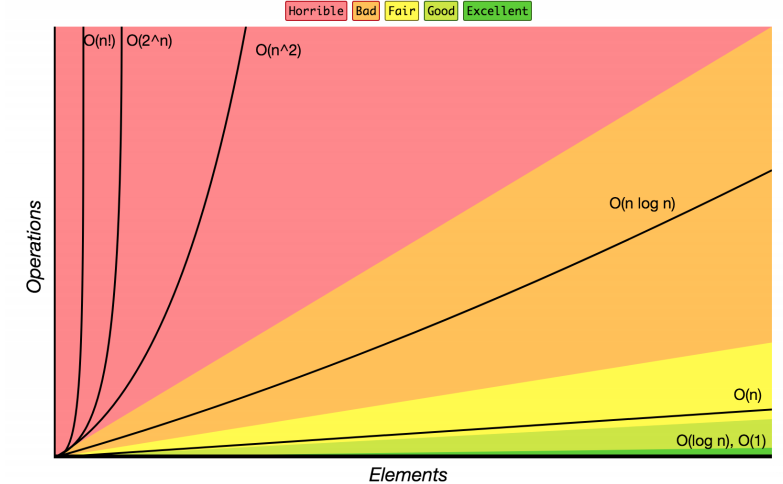
\includegraphics[width=\linewidth,height=\textheight, keepaspectratio]{extracted_media/image_1.png}
  \end{minipage}
\end{textblock}
\begin{textblock}{0.431}(0.554, 0.363)
  \begin{minipage}[t][0.495\paperheight]{\linewidth}
    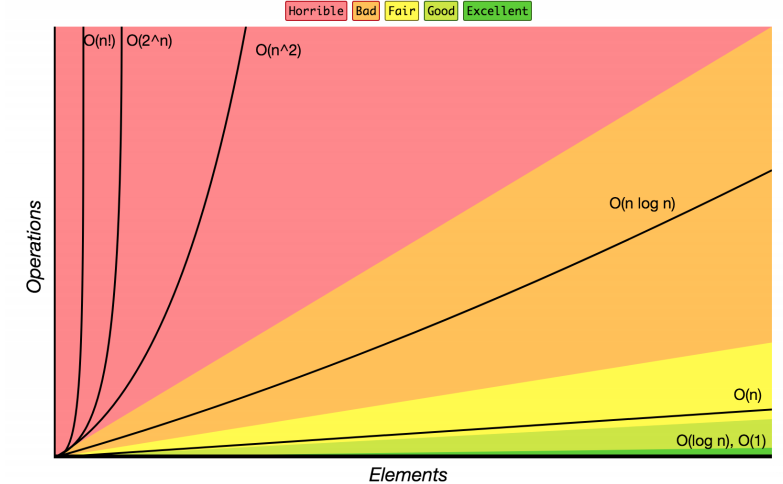
\includegraphics[width=\linewidth,height=\textheight, keepaspectratio]{extracted_media/image_1.png}
  \end{minipage}
\end{textblock}
\end{frame}

% --- Slide 3 ---
\begin{frame}[fragile]
\begin{textblock}{0.886}(0.099, 0.076)
  \begin{minipage}[t][0.131\paperheight]{\linewidth}
    \textbf{Code Modellierung Beispiel 2}
  \end{minipage}
\end{textblock}
\begin{textblock}{0.885}(0.099, 0.022)
  \begin{minipage}[b][0.031\paperheight]{\linewidth}
    \raggedright
    \fontsize{3}{3.3}\selectfont Algorithmik – Laufzeitanalyse von Algorithmen durch Asymptotische Notation
  \end{minipage}
\end{textblock}
\begin{textblock}{0.042}(0.309, 0.27)
  \begin{minipage}[t][0.044\paperheight]{\linewidth}
    {\tiny +1}
  \end{minipage}
\end{textblock}
\begin{textblock}{0.042}(0.288, 0.317)
  \begin{minipage}[t][0.044\paperheight]{\linewidth}
    {\tiny +1}
  \end{minipage}
\end{textblock}
\begin{textblock}{0.042}(0.351, 0.361)
  \begin{minipage}[t][0.044\paperheight]{\linewidth}
    {\tiny +1}
  \end{minipage}
\end{textblock}
\begin{textblock}{0.042}(0.483, 0.497)
  \begin{minipage}[t][0.044\paperheight]{\linewidth}
    {\tiny +2}
  \end{minipage}
\end{textblock}
\begin{textblock}{0.042}(0.319, 0.813)
  \begin{minipage}[t][0.044\paperheight]{\linewidth}
    {\tiny +1}
  \end{minipage}
\end{textblock}
\begin{textblock}{0.042}(0.631, 0.575)
  \begin{minipage}[t][0.044\paperheight]{\linewidth}
    {\tiny +9}
  \end{minipage}
\end{textblock}
\begin{textblock}{0.035}(0.627, 0.529)
  \begin{minipage}[t][0.054\paperheight]{\linewidth}
    {\tiny *n\\*n}
  \end{minipage}
\end{textblock}
\begin{textblock}{0.15}(0.624, 0.456)
  \begin{minipage}[t][0.094\paperheight]{\linewidth}
    {\tiny Innere Schleife läuft n-mal}
  \end{minipage}
\end{textblock}
\begin{textblock}{0.238}(0.704, 0.142)
  \begin{minipage}[t][0.168\paperheight]{\linewidth}
    {\tiny f(n) = (9n+4)n + 3}
  \end{minipage}
\end{textblock}
\begin{textblock}{0.042}(0.339, 0.409)
  \begin{minipage}[t][0.044\paperheight]{\linewidth}
    {\tiny +1}
  \end{minipage}
\end{textblock}
\begin{textblock}{0.042}(0.405, 0.451)
  \begin{minipage}[t][0.044\paperheight]{\linewidth}
    {\tiny +1}
  \end{minipage}
\end{textblock}
\begin{textblock}{0.042}(0.393, 0.677)
  \begin{minipage}[t][0.044\paperheight]{\linewidth}
    {\tiny +2}
  \end{minipage}
\end{textblock}
\begin{textblock}{0.042}(0.331, 0.765)
  \begin{minipage}[t][0.044\paperheight]{\linewidth}
    {\tiny +2}
  \end{minipage}
\end{textblock}
\begin{textblock}{0.042}(0.539, 0.631)
  \begin{minipage}[t][0.044\paperheight]{\linewidth}
    {\tiny +4}
  \end{minipage}
\end{textblock}
\begin{textblock}{0.083}(0.819, 0.562)
  \begin{minipage}[t][0.044\paperheight]{\linewidth}
    {\tiny 9n + 4}
  \end{minipage}
\end{textblock}
\begin{textblock}{0.143}(0.843, 0.446)
  \begin{minipage}[t][0.094\paperheight]{\linewidth}
    {\tiny Äußere Schleife läuft n-mal}
  \end{minipage}
\end{textblock}
\begin{textblock}{0.886}(0.099, 0.226)
  \begin{minipage}[t][0.63\paperheight]{\linewidth}
    \begin{lstlisting}[language=Java, basicstyle=\ttfamily\scriptsize]
public int method2(int n) {
int sum = 0;
int i = 0;
while (i < n) {
int j = 0;
while (j < n) {
if (j % 2 == 0) {
// do nothing
}
sum = sum + (i * 3) + j;
j = j + 1;
}
i = i + 1;
} return sum;
}
    \end{lstlisting}
  \end{minipage}
\end{textblock}
\begin{textblock}{0.106}(0.099, 0.877)
  \begin{minipage}[b][0.026\paperheight]{\linewidth}
    \raggedright
    \fontsize{3}{3.3}\selectfont 06.03.2026
  \end{minipage}
\end{textblock}
\begin{textblock}{0.106}(0.099, 0.928)
  \begin{minipage}[b][0.031\paperheight]{\linewidth}
    \raggedright
    \fontsize{3}{3.3}\selectfont Seite 3
  \end{minipage}
\end{textblock}
\begin{textblock}{0.231}(0.564, 0.897)
  \begin{minipage}[b][0.032\paperheight]{\linewidth}
    \raggedright
    \fontsize{3}{3.3}\selectfont Quelle: Data Structures and Algorithms (CSE 373), University of Washington, Spring 2022
  \end{minipage}
\end{textblock}
\begin{textblock}{0.18}(0.615, 0.934)
  \begin{minipage}[b][0.032\paperheight]{\linewidth}
    \raggedright
    \fontsize{3}{3.3}\selectfont CSE 373 20 AU – SCHAFER
  \end{minipage}
\end{textblock}
\end{frame}

% --- Slide 4 ---
\begin{frame}[fragile]
\begin{textblock}{0.512}(0.473, 0.587)
  \begin{minipage}[t][0.064\paperheight]{\linewidth}
    {\tiny Θ-Notation}
  \end{minipage}
\end{textblock}
\begin{textblock}{0.886}(0.099, 0.076)
  \begin{minipage}[t][0.131\paperheight]{\linewidth}
    \textbf{O-, Ω- und Θ-Notation Übung}
  \end{minipage}
\end{textblock}
\begin{textblock}{0.886}(0.099, 0.226)
  \begin{minipage}[t][0.63\paperheight]{\linewidth}
    {\small Welche der folgenden Funktionen ist in O(n²)? Ω(n²)? Θ(n²)?}
  \end{minipage}
\end{textblock}
\begin{textblock}{0.885}(0.099, 0.022)
  \begin{minipage}[b][0.031\paperheight]{\linewidth}
    \fontsize{3}{3.3}\selectfont
    \textbf{Algorithmik – Laufzeitanalyse von Algorithmen durch Asymptotische Notation}
  \end{minipage}
\end{textblock}
\begin{textblock}{0.03}(0.1, 0.286)
  \begin{minipage}[t][0.054\paperheight]{\linewidth}
    {\tiny a.}
  \end{minipage}
\end{textblock}
\begin{textblock}{0.03}(0.1, 0.399)
  \begin{minipage}[t][0.054\paperheight]{\linewidth}
    {\tiny b.}
  \end{minipage}
\end{textblock}
\begin{textblock}{0.028}(0.1, 0.498)
  \begin{minipage}[t][0.054\paperheight]{\linewidth}
    {\tiny c.}
  \end{minipage}
\end{textblock}
\begin{textblock}{0.03}(0.1, 0.612)
  \begin{minipage}[t][0.054\paperheight]{\linewidth}
    {\tiny d.}
  \end{minipage}
\end{textblock}
\begin{textblock}{0.03}(0.1, 0.722)
  \begin{minipage}[t][0.054\paperheight]{\linewidth}
    {\tiny e.}
  \end{minipage}
\end{textblock}
\begin{textblock}{0.132}(0.12, 0.342)
  \begin{minipage}[t][0.054\paperheight]{\linewidth}
    {\tiny f(n) ∈ O(n2)}
  \end{minipage}
\end{textblock}
\begin{textblock}{0.129}(0.12, 0.45)
  \begin{minipage}[t][0.054\paperheight]{\linewidth}
    {\tiny f(n) ∈ O(n2)}
  \end{minipage}
\end{textblock}
\begin{textblock}{0.132}(0.12, 0.553)
  \begin{minipage}[t][0.054\paperheight]{\linewidth}
    {\tiny f(n) ∈ O(n2)}
  \end{minipage}
\end{textblock}
\begin{textblock}{0.124}(0.12, 0.675)
  \begin{minipage}[t][0.054\paperheight]{\linewidth}
    {\tiny f(n) ∈ O(n2)}
  \end{minipage}
\end{textblock}
\begin{textblock}{0.116}(0.235, 0.677)
  \begin{minipage}[t][0.054\paperheight]{\linewidth}
    {\tiny f(n) ∈ Ω(n2)}
  \end{minipage}
\end{textblock}
\begin{textblock}{0.122}(0.122, 0.786)
  \begin{minipage}[t][0.054\paperheight]{\linewidth}
    {\tiny f(n) ∈ Ω(n2)}
  \end{minipage}
\end{textblock}
\begin{textblock}{0.116}(0.353, 0.677)
  \begin{minipage}[t][0.054\paperheight]{\linewidth}
    {\tiny f(n) ∈ Θ(n2)}
  \end{minipage}
\end{textblock}
\begin{textblock}{0.18}(0.615, 0.934)
  \begin{minipage}[b][0.032\paperheight]{\linewidth}
    \raggedright
    \fontsize{3}{3.3}\selectfont
    CSE 373 20 SP – CHUN & CHAMPION
  \end{minipage}
\end{textblock}
\begin{textblock}{0.231}(0.564, 0.897)
  \begin{minipage}[b][0.032\paperheight]{\linewidth}
    \raggedright
    \fontsize{3}{3.3}\selectfont
    Quelle: Data Structures and Algorithms (CSE 373), University of Washington, Spring 2022
  \end{minipage}
\end{textblock}
\begin{textblock}{0.375}(0.609, 0.066)
  \begin{minipage}[t][0.064\paperheight]{\linewidth}
    {\tiny O-Notation}
  \end{minipage}
\end{textblock}
\begin{textblock}{0.375}(0.609, 0.329)
  \begin{minipage}[t][0.064\paperheight]{\linewidth}
    {\tiny Ω-Notation}
  \end{minipage}
\end{textblock}
\begin{textblock}{0.106}(0.099, 0.877)
  \begin{minipage}[b][0.026\paperheight]{\linewidth}
    \raggedright
    \fontsize{3}{3.3}\selectfont
    06.03.2026
  \end{minipage}
\end{textblock}
\begin{textblock}{0.106}(0.099, 0.928)
  \begin{minipage}[b][0.031\paperheight]{\linewidth}
    \raggedright
    \fontsize{3}{3.3}\selectfont
    Seite 4
  \end{minipage}
\end{textblock}
\begin{textblock}{0.368}(0.613, 0.394)
  \begin{minipage}[t][0.164\paperheight]{\linewidth}
    
\includegraphics[width=\linewidth, height=\textheight, keepaspectratio]{extracted_media/image_2.png}
  \end{minipage}
\end{textblock}
\begin{textblock}{0.368}(0.613, 0.394)
  \begin{minipage}[t][0.164\paperheight]{\linewidth}
    
\includegraphics[width=\linewidth, height=\textheight, keepaspectratio]{extracted_media/image_2.png}
  \end{minipage}
\end{textblock}
\begin{textblock}{0.375}(0.609, 0.131)
  \begin{minipage}[t][0.166\paperheight]{\linewidth}
    
\includegraphics[width=\linewidth, height=\textheight, keepaspectratio]{extracted_media/image_3.png}
  \end{minipage}
\end{textblock}
\begin{textblock}{0.375}(0.609, 0.131)
  \begin{minipage}[t][0.166\paperheight]{\linewidth}
    
\includegraphics[width=\linewidth, height=\textheight, keepaspectratio]{extracted_media/image_3.png}
  \end{minipage}
\end{textblock}
\begin{textblock}{0.512}(0.473, 0.652)
  \begin{minipage}[t][0.209\paperheight]{\linewidth}
    
\includegraphics[width=\linewidth, height=\textheight, keepaspectratio]{extracted_media/image_4.png}
  \end{minipage}
\end{textblock}
\begin{textblock}{0.512}(0.473, 0.652)
  \begin{minipage}[t][0.209\paperheight]{\linewidth}
    
\includegraphics[width=\linewidth, height=\textheight, keepaspectratio]{extracted_media/image_4.png}
  \end{minipage}
\end{textblock}
\end{frame}


\end{document}
